\documentclass{article}
\usepackage[utf8]{inputenc} % allow utf-8 input
\usepackage[T1]{fontenc}    % use 8-bit T1 fonts
\usepackage{hyperref}       % hyperlinks
\usepackage{url}            % simple URL typesetting
\usepackage{booktabs}       % professional-quality tables
\usepackage{amsfonts}       % blackboard math symbols
\usepackage{nicefrac}       % compact symbols for 1/2, etc.
\usepackage{microtype}      % microtypography
\usepackage{mathptmx}
\usepackage{xcolor}         % colors
\usepackage[left=1.5in, right=1.5in, top=1in]{geometry}
\usepackage{graphicx}
\usepackage{float}
\usepackage{placeins}
\usepackage{amsmath}
\usepackage[skip=0.5\baselineskip]{caption}

 \author{
  \textbf{Ding, Ma}\\
  Boston University
  \and
  \textbf{Hank, Zhong}\\  
  Boston University
  \and
 \textbf{Yifan, Zhang}\\ 
 Boston University
}
\title{\rule{\textwidth}{4pt}\\\textbf{Prediction on the Churn through Classification}\\\rule{\textwidth}{1pt}}
\begin{document}
\maketitle
\begin{abstract}
  Any business wants to maximize the number of customers. In this paper, we approach a model, based on a dataset from a telecommunications company, to predict the customer churn in order to create a chance for company to retain old clients. The accuracy of our model is close related to cost of the retaining, so in order to get higher accuracy we have to deal with two challenges: missing data and imbalanced data. For missing data, we use either replacing missing data with mean or directly deleting it, and the result demonstrate higher accuracy for deleting method. The major challenge comes from the imbalance, and in order to increase the accuracy, we implement four methods: Penalization on the target class, Decreasing the threshold, Oversampling, and Undersampling. According to the result, Penalization on the target class has highest accuracy for the prediction of the customer churn, and it leads to more effective cost of companies.
\end{abstract}
\section{Data Set Analysis}
\subsection{Missing Dataset}	
Before building a model, we analyze the dataset in order to find out the potential cause of bias. After factorizing categorical data and converting string-format real value to float format, we figure out that 10 users has missing data. To minimize the influence of missing data, we implement two method. First one is replacing missing data with mean, and second one is deleting all the missing values. 
\FloatBarrier
\begin{table}[htb]
\centering
\caption{Accuracy of the method for the missing data}
	\begin{tabular}{||c c c c c||} 
	 \hline
 	Method & Churn & Precision & Recall & F1-score  \\ [0.5ex] 
 	\hline\hline
   	& False (Not churn) & 0.85 & 0.98 & 0.87 \\ 
  	Replacing & True (Churn) & 0.61 & 0.52 & 0.56 \\
   	& average & 0.79 & 0.79 & 0.79 \\
   	\hline
  	& False (Not churn) & 0.85 & 0.91 & 0.88 \\
 	Deleting & True (Churn) & 0.67 & 0.53 & 0.59 \\
  	& average & 0.80 & 0.81 & 0.80 \\ [1ex] 
 	\hline
	\end{tabular}
\label{missing}
\end{table}
\FloatBarrier

\noindent Shown as Table \ref{missing}, we use three values, precision, recall and F1-score to determine the accuracy for each level of two methods. Precision gives the ratio of correctly predicted positive observations to the total predicted positive observations. Recall shows the ratio of correctly predicted positive observations to the all observations in actual class - churn. F1-score is the weighted average of Precision and Recall. From the Table \ref{missing}, the result clearly demonstrates that when the missing value is not extremely large, deletion is the better way to deal with the missing data.
\subsection{Imbalanced Data}
The other challenge in the dataset is the imbalanced data. Shown as Figure \ref{fig:imbalanced}, we have more data on stable customers than leaving customers. This may lead our model to classify not leaving customers more frequently since there are more data to be trained than leaving customers, and it might cause the extra loss of company. Assuming a customer has high probability to leave the service(churn) ,but if our model's prediction excludes him or her from the customer churn which is False Negative. The company will not focus on that customer's services, then this customer will definitely leave the services(churn), which results a customer loss of the company. In the other situation, if a customer is not willing to leave the services and is satisfied, but our model gives the opposite result, then the company will provide this customer extra benefits. This causes the wasted investment of the company. Therefore, other than focusing on the increment of recall or precision, we will use F1-score as the evaluation of the model.
\FloatBarrier
\begin{figure}[htb]
    \centering
    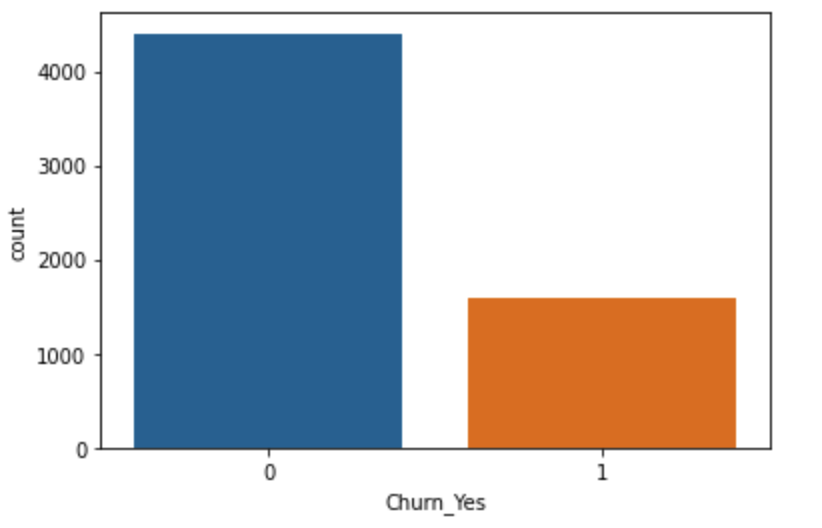
\includegraphics[width=7.5cm]{imbalanced}
    \caption{Imbalanced of the dataset}
    \label{fig:imbalanced}
\end{figure}
\FloatBarrier
\section{Models}
\subsection{Normal Logistic Regression}
Since our numerical data have various range and unknown distribution, before training the model, we implement normalization with the function:
\[x = \frac{x - \bar{x}}{\sigma}\texttt{,}\]
in which $\bar{x}$ is the mean and $\sigma$ is the standard deviation.
\vspace{5.5pt}

\noindent Then we apply the dataset in to logistic regression, and the function return the result as Table \ref{NLR}. The accuracy of the model is 0.81, which seems like to a satisfied result. However, when we check the accuracy and recall of different classes, churn and not churn, the result shows that both values of determining the leaving customer are lower than 0.7. Therefore, we need to increase the model’s False Negative rate while maintaining the overall performance to prevent the loss of companies mentioned in previous section.
\FloatBarrier
\begin{table}[htb]
\centering
\caption{Accuracy of the normal Logistic Regression}
	\begin{tabular}{||c c c c ||} 
	 \hline
 	Churn & Precision & Recall & F1-score  \\ [0.5ex] 
 	\hline\hline
 	False (Not churn) & 0.85 & 0.91 & 0.88 \\ 
 	True (Churn) & 0.67 & 0.53 & 0.59 \\
   	average & 0.80 & 0.81 & 0.80 \\
 	\hline
	\end{tabular}
\label{NLR}
\end{table}
\FloatBarrier
\subsection{L2 Penalization}
Due to the imbalanced property of our dataset, the training model appears to have higher frequency on classifying 0 (not churn). Therefore, we try to add L2 penalization on target class so that the classifier are forced to classify more 1s (churn) than 0, in order to increase the recall of classifying 1. The error function with L2 penalization is 
\[E(w)=-[y*ln(\hat{y})+(l-y)*ln(1-\hat{y})]+\lambda*(1-y)^2\texttt{,}\]
where $\lambda$ represents for penalty. According to this error function, we derive new back propagation equations for weights and bias, such as
\begin{align*}
\frac{\partial E(w)}{\partial \hat{y}} &= -[\frac{y}{\hat{y}}-\frac{1-y}{•1-\hat{y}}]-2\lambda*(1-\hat{y})\\
\frac{\partial E(w)}{\partial w} &=  \frac{\partial E(w)}{\partial \hat{y}} * \frac{\partial \hat{y}}{\partial w} \\
											&= [-[\frac{y}{\hat{y}}-\frac{1-y}{1-\hat{y}}]-2\lambda*(1-\hat{y}*[\frac{\partial}{\partial w}(\sigma(w*x))] \\
											&= [\hat{y}-y-2\lambda*\hat{y}*(1-\hat{y})^2]*x^T
\end{align*}
After we use this back propagation formula to update the original logistic regression model, the result changes as we want. In order to improve the model, we try different punishment intensity and form a graph according to the corresponding values of model's True recall and True F1-score. 
\FloatBarrier
\begin{figure}[htb]
    \centering
    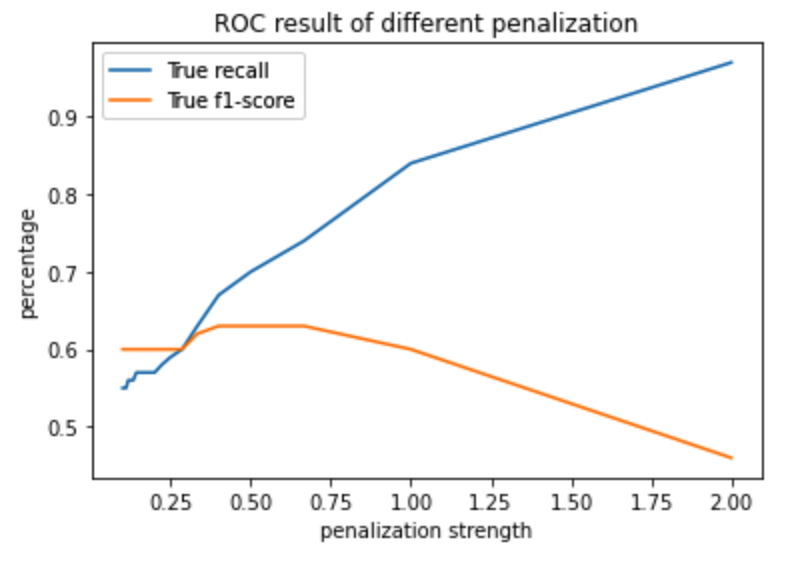
\includegraphics[width=7.5cm]{ROC_penalization}
    \caption{ROC of different penalty strength}
    \label{fig:penalty}
\end{figure}
\FloatBarrier
Shown by Figure \ref{fig:penalty}, the best choice of penalty strength should be 0.666, so we determine $\lambda$ value in our previous error function to be 0.666, and recalculate the accuracy of the model, which is shown in Table \ref{penalty}.
\FloatBarrier
\begin{table}[htb]
\centering
\caption{Accuracy of L2 penalization on the target class}
	\begin{tabular}{||c c c c ||} 
	 \hline
 	Churn & Precision & Recall & F1-score  \\ [0.5ex] 
 	\hline\hline
 	False (Not churn) & 0.90 & 0.91 & 0.88 \\ 
 	True (Churn) & 0.54 & 0.74 & 0.63 \\
   	average & 0.80 & 0.77 & 0.78 \\
 	\hline
	\end{tabular}
\label{penalty}
\end{table}
\FloatBarrier
\subsection{Oversampling and Undersampling}
\subsubsection{Oversampling}
The other idea of minimize the bias caused by the imbalanced dataset is to manually change the proportion of different classes through either Oversampling or Undersampling. 
\vspace{5.5pt}

\noindent Oversampling is usually achieved by repeatedly sampling the minority class, which is the churn class in our case, but simple repetition is likely to lead to overfitting of the model. Therefore, we use the SMOTE, Synthetic Minority Oversampling Techniques, as an improvement, which can effectively reduce overfitting by synthesizing new samples with fewer categories through k-nearest neighbors in the local area. After we implement SMOTE, sizes of two class, churn and not churn, become the same, which is shown as Figure \ref{fig:oversampling}.
\FloatBarrier
\begin{figure}[htb]
    \centering
    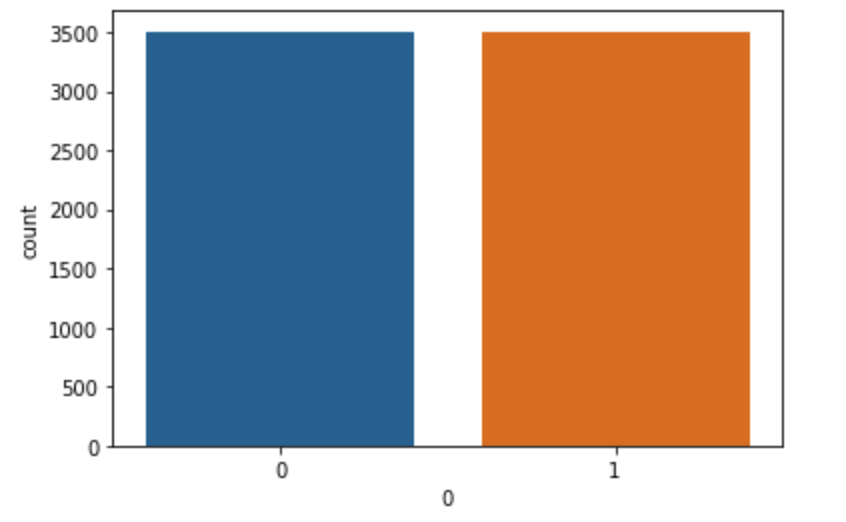
\includegraphics[width=7.5cm]{Oversampling}
    \caption{Oversampling}
    \label{fig:oversampling}
\end{figure}
\FloatBarrier

\subsubsection{Undersampling}
Undersampling is to balance the sample size of different categories by randomly deleting samples from majority class. However, the number of samples in this dataset is not very large. If too many samples are discarded, the recognition accuracy of the model for the categories with more samples will decline. So we plan to use multiple under sampling, then train multiple models, and finally use voting to determine the final prediction results. After implementing Undersampling, shown as Figure \ref{fig:undersampling}, the size of majority class decrease to the same level as the minority class. 
\FloatBarrier
\begin{figure}[htb]
    \centering
    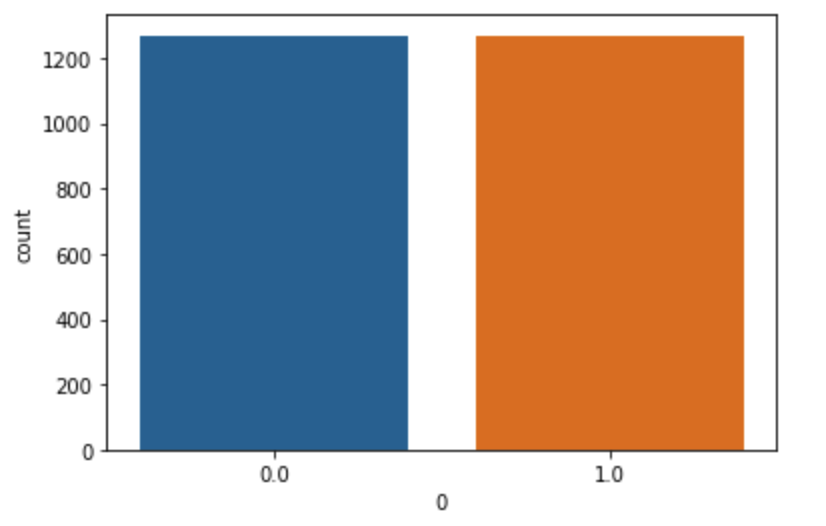
\includegraphics[width=7.5cm]{Undersampling}
    \caption{Undersampling}
    \label{fig:undersampling}
\end{figure}
\FloatBarrier

\noindent The accuracy table of undersampling and oversampling is shown as Table \ref{Accucray of Oversampling and Undersampling}, and it shows that even undersampling uses a smaller proportion of data, the result is better than oversampling. One reason of this is that oversampling more or less causes overfitting which may affect the accuracy of the model when validation uses the test set.
\FloatBarrier
\begin{table}[htb]
\centering
\caption{Accuracy of the method for the missing data}
	\begin{tabular}{||c c c c c||} 
	 \hline
 	Method & Churn & Precision & Recall & F1-score  \\ [0.5ex] 
 	\hline\hline
   	& False (Not churn) & 0.91 & 0.76 & 0.83 \\ 
  	Oversampling & True (Churn) & 0.54 & 0.79 & 0.64 \\
   	& average & 0.81 & 0.77 & 0.78 \\
   	\hline
  	& False (Not churn) & 0.91 & 0.78 & 0.84 \\
 	Undersampling & True (Churn) & 0.56 & 0.78 & 0.66 \\
  	& average & 0.82 & 0.78 & 0.79 \\ [1ex] 
 	\hline
	\end{tabular}
\label{Accucray of Oversampling and Undersampling}
\end{table}
\FloatBarrier

\subsection{Decreasing Threshold}
Another way of minimizing the bias from the imbalanced data is simply changing the threshold when predicting using the output of the ordinary logistic regression, as shown in the following function.
\[ class = \begin{cases} 
      			0 & \hat{y}> threshold \\
      			1 & \hat{y}\leq threshold 
  			   \end{cases}
\]
Shown as Figure \ref{fig:threshold}, when the threshold value roughly around 0.3 to 0.4, True recall and True F1-score is balanced. After we multiple attempts on changing threshold between this interval, 0.333 gives our best feedback on the accuracy, shown as Table \ref{threshold}.
\FloatBarrier
\begin{figure}[htb]
\centering
    \includegraphics[width=7.5cm]{Threshold}
    \caption{ROC of threshold}
    \label{fig:threshold}
\end{figure}
\FloatBarrier
\begin{table}[htb]
\centering
\caption{Accuracy of threshold value 0.333}
	\begin{tabular}{||c c c c ||} 
	 \hline
 	Churn & Precision & Recall & F1-score  \\ [0.5ex] 
 	\hline\hline
 	False (Not churn) & 0.89 & 0.79 & 0.84 \\ 
 	True (Churn) & 0.55 & 0.73 & 0.63 \\
   	average & 0.80 & 0.77 & 0.78 \\
 	\hline
	\end{tabular}\label{threshold}
\end{table}
\FloatBarrier

\section{Conclusion}
After we implement four methods to overcome the major challenge, the imbalance, we use value of recall and F1-score as the evaluation standard. From Table  \ref{all}, the penalization method has the maximum False F1-score, minimum variance, and close values on other measurements, which means that this method has high accuracy and does generalization on the data. Therefore, the method of penalization is the best way among the others to minimize the bias of the imbalanced data. 
\FloatBarrier
\begin{table}[htb]
\centering
\caption{The accuracy of all four methods}
	\begin{tabular}{||c c c c c c||} 
	 \hline
 	Method & True recall & True F1-score  & False F1-score & Model F1-score & variance\\ [0.5ex] 
 	\hline\hline
 	Original & 0.53 & 0.59 & 0.88 & 0.80 &  \\ 
 	Penalization & 0.74 & 0.63 & 0.88 & 0.78 & 0.03366\\
   	Oversampling & 0.79 & 0.64 & 0.83 & 0.78 & \\
   	Undersampling & 0.78 & 0.66 & 0.84 & 0.79 & \\
   	Threshold & 0.73 & 0.64 & 0.83 & 0.78 & 0.12487\\
 	\hline
	\end{tabular}
\label{all}
\end{table}
\FloatBarrier
\end{document}


